\documentclass[border=8pt]{standalone}
\usepackage{tikz}
\usetikzlibrary{shapes.geometric, arrows.meta, positioning, fit, backgrounds, calc}
\usepackage{xcolor}

% Paul Tol bright palette — colorblind-safe
\definecolor{wfinput}{HTML}{CCBB44}
\definecolor{wfprocess}{HTML}{4477AA}
\definecolor{wfintermediate}{HTML}{66CCEE}
\definecolor{wfhardware}{HTML}{EE6677}
\definecolor{wfoutput}{HTML}{228833}
\definecolor{wfside}{HTML}{AA3377}
% Group box colors
\definecolor{wfgroup1}{HTML}{BBBBCC}
\definecolor{wfgroup2}{HTML}{BBCCBB}
\definecolor{wfgroup3}{HTML}{CCBBBB}

\begin{document}
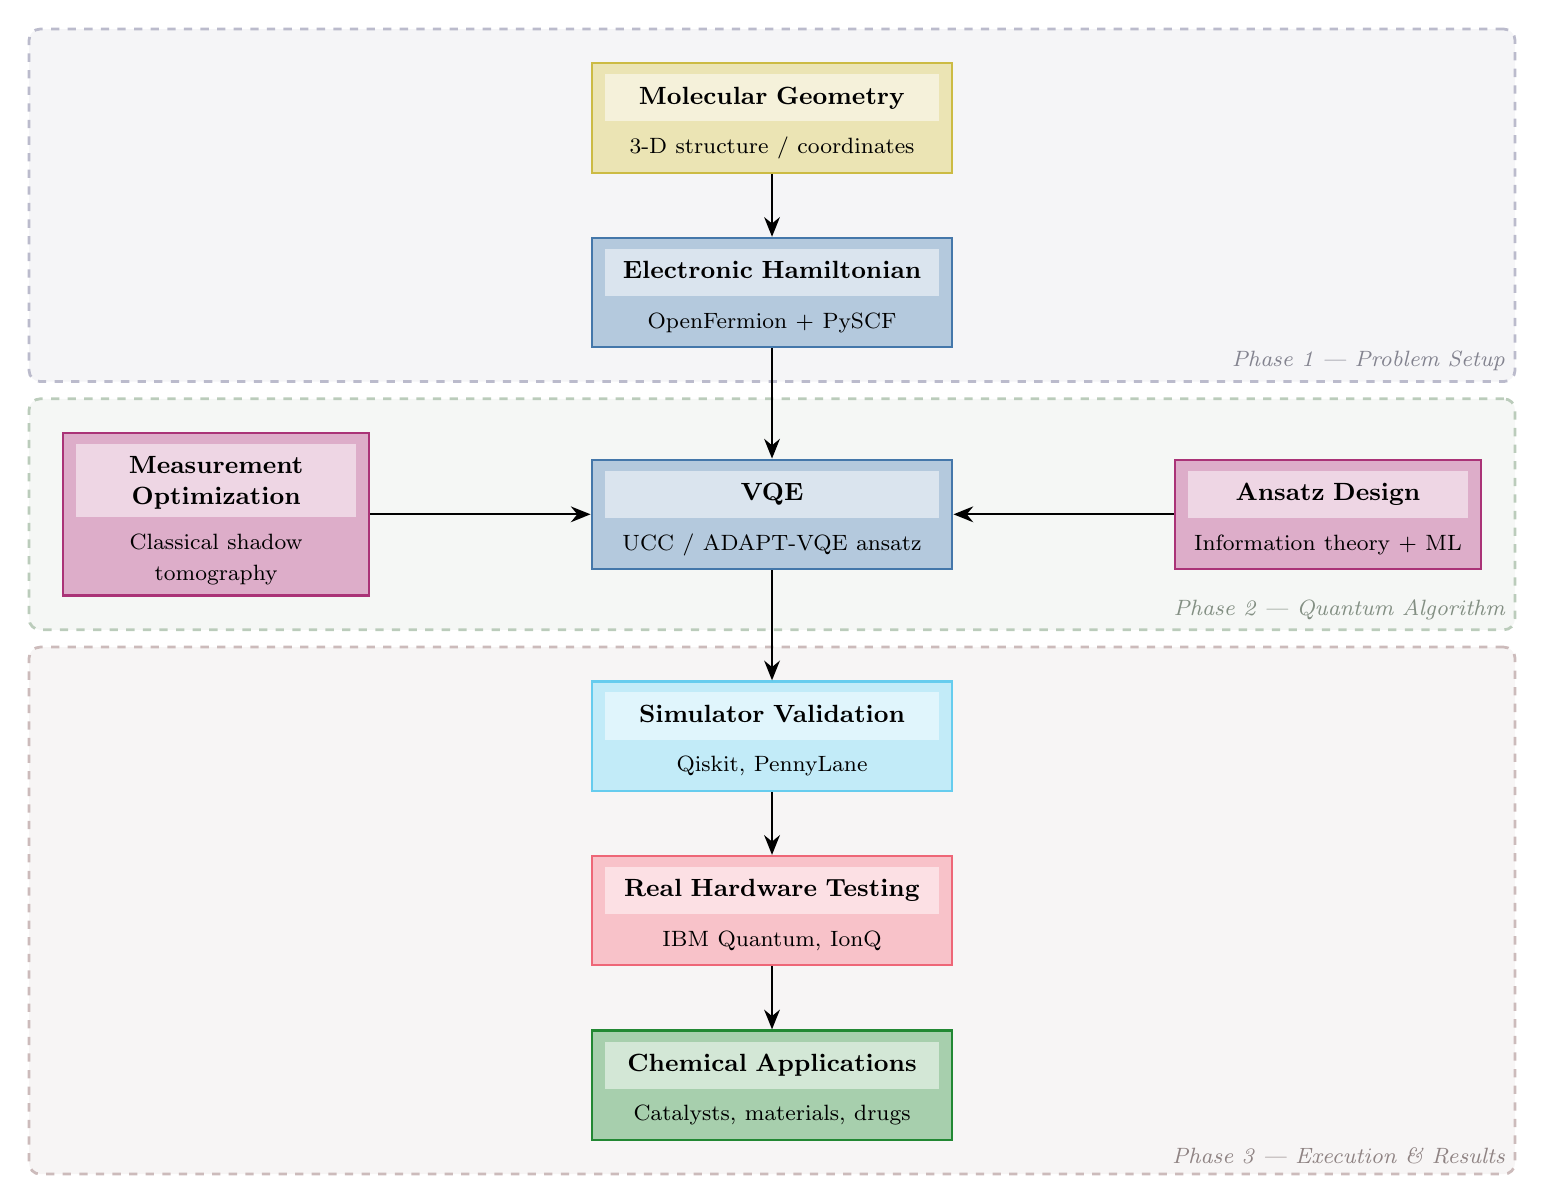
\begin{tikzpicture}[
    node distance=0.8cm and 2.8cm,
    every node/.style={align=center, font=\small},
    wf-input/.style={rectangle,
        minimum width=4.5cm, text width=4.3cm,
        draw=wfinput, line width=0.8pt, fill=wfinput!40, inner sep=4pt},
    wf-process/.style={rectangle,
        minimum width=4.5cm, text width=4.3cm,
        draw=wfprocess, line width=0.8pt, fill=wfprocess!40, inner sep=4pt},
    wf-intermediate/.style={rectangle,
        minimum width=4.5cm, text width=4.3cm,
        draw=wfintermediate, line width=0.8pt, fill=wfintermediate!40, inner sep=4pt},
    wf-hardware/.style={rectangle,
        minimum width=4.5cm, text width=4.3cm,
        draw=wfhardware, line width=0.8pt, fill=wfhardware!40, inner sep=4pt},
    wf-output/.style={rectangle,
        minimum width=4.5cm, text width=4.3cm,
        draw=wfoutput, line width=0.8pt, fill=wfoutput!40, inner sep=4pt},
    wf-side/.style={rectangle,
        minimum width=3.8cm, text width=3.6cm,
        draw=wfside, line width=0.8pt, fill=wfside!40, inner sep=4pt},
    wf-arrow/.style={-{Stealth[length=2.5mm, width=2mm]}, thick},
]
    % ---- NODES: main chain ----
    % Phase 1: geom, hamil
    \node[wf-input] (geom) {%
        {\setlength{\fboxsep}{3pt}%
         \colorbox{wfinput!20}{\parbox{4.04cm}{\centering\strut\textbf{Molecular Geometry}}}}\\[4pt]
        {\footnotesize\strut 3-D structure / coordinates}};

    \node[wf-process, below=0.8cm of geom] (hamil) {%
        {\setlength{\fboxsep}{3pt}%
         \colorbox{wfprocess!20}{\parbox{4.04cm}{\centering\strut\textbf{Electronic Hamiltonian}}}}\\[4pt]
        {\footnotesize\strut OpenFermion + PySCF}};

    % Phase 2: vqe (+ side branches) — 1.4cm gap at phase boundary
    \node[wf-process, below=1.4cm of hamil] (vqe) {%
        {\setlength{\fboxsep}{3pt}%
         \colorbox{wfprocess!20}{\parbox{4.04cm}{\centering\strut\textbf{VQE}}}}\\[4pt]
        {\footnotesize\strut UCC / ADAPT-VQE ansatz}};

    % Phase 3: sim, hw, apps — 1.4cm gap at phase boundary
    \node[wf-intermediate, below=1.4cm of vqe] (sim) {%
        {\setlength{\fboxsep}{3pt}%
         \colorbox{wfintermediate!20}{\parbox{4.04cm}{\centering\strut\textbf{Simulator Validation}}}}\\[4pt]
        {\footnotesize\strut Qiskit, PennyLane}};

    \node[wf-hardware, below=0.8cm of sim] (hw) {%
        {\setlength{\fboxsep}{3pt}%
         \colorbox{wfhardware!20}{\parbox{4.04cm}{\centering\strut\textbf{Real Hardware Testing}}}}\\[4pt]
        {\footnotesize\strut IBM Quantum, IonQ}};

    \node[wf-output, below=0.8cm of hw] (apps) {%
        {\setlength{\fboxsep}{3pt}%
         \colorbox{wfoutput!20}{\parbox{4.04cm}{\centering\strut\textbf{Chemical Applications}}}}\\[4pt]
        {\footnotesize\strut Catalysts, materials, drugs}};

    % ---- NODES: side branches (at vqe level) ----
    \node[wf-side, right=2.8cm of vqe] (ansatz) {%
        {\setlength{\fboxsep}{3pt}%
         \colorbox{wfside!20}{\parbox{3.34cm}{\centering\strut\textbf{Ansatz Design}}}}\\[4pt]
        {\footnotesize\strut Information theory + ML}};

    \node[wf-side, left=2.8cm of vqe] (measopt) {%
        {\setlength{\fboxsep}{3pt}%
         \colorbox{wfside!20}{\parbox{3.34cm}{\centering\strut\textbf{Measurement Optimization}}}}\\[4pt]
        {\footnotesize\strut Classical shadow tomography}};

    % ---- GROUP BOXES (full diagram width, background layer) ----
    % Capture diagram extent after all nodes, before group boxes:
    \coordinate (bb-w) at (current bounding box.west);
    \coordinate (bb-e) at (current bounding box.east);

    \begin{scope}[on background layer]
        \node[draw=wfgroup1, dashed, line width=1pt, rounded corners=4pt,
              fill=wfgroup1!15, inner sep=12pt,
              fit=(bb-w |- geom.north)(bb-e |- hamil.south)] (grp1) {};
    \end{scope}
    \node[text=wfgroup1!70!black, font=\footnotesize\itshape, anchor=south east, inner sep=4pt]
        at (grp1.south east) {Phase 1 --- Problem Setup};

    \begin{scope}[on background layer]
        \node[draw=wfgroup2, dashed, line width=1pt, rounded corners=4pt,
              fill=wfgroup2!15, inner sep=12pt,
              fit=(bb-w |- vqe.north)(bb-e |- vqe.south)(measopt)(ansatz)] (grp2) {};
    \end{scope}
    \node[text=wfgroup2!70!black, font=\footnotesize\itshape, anchor=south east, inner sep=4pt]
        at (grp2.south east) {Phase 2 --- Quantum Algorithm};

    \begin{scope}[on background layer]
        \node[draw=wfgroup3, dashed, line width=1pt, rounded corners=4pt,
              fill=wfgroup3!15, inner sep=12pt,
              fit=(bb-w |- sim.north)(bb-e |- apps.south)] (grp3) {};
    \end{scope}
    \node[text=wfgroup3!70!black, font=\footnotesize\itshape, anchor=south east, inner sep=4pt]
        at (grp3.south east) {Phase 3 --- Execution \& Results};

    % ---- ARROWS: main chain ----
    \draw[wf-arrow] (geom)  -- (hamil);
    \draw[wf-arrow] (hamil) -- (vqe);
    \draw[wf-arrow] (vqe)   -- (sim);
    \draw[wf-arrow] (sim)   -- (hw);
    \draw[wf-arrow] (hw)    -- (apps);

    % ---- ARROWS: side inputs into VQE ----
    \draw[wf-arrow] (ansatz)  -- (vqe);
    \draw[wf-arrow] (measopt) -- (vqe);

\end{tikzpicture}
\end{document}
